\chapter{Engineering Analysis}

Once design alternatives were evaluated and the anticipated project implementation specifics were chosen, the team set out to professionally implement the design.
This entails carefully designing each of the project's components, including the hardware design, software design, and packaging design.
Thorough design ensured that implementation issues were anticipated and therefore mitigated or avoided.

\section{Packaging Design}
\subsection{Overview}
Packaging for the \gls{ceenc} was constructed primarily from laser cut acrylic, as shown below. 
Laser cutting services were provided by Pokono, for a materials fee and machinery surcharge.
Design of the packaging was completed utilizing InkScape Vector Design Software.
Measurements were taken from the Master, Controller, and Driver boards, then translated into cutouts to support the components.
These cutouts were attatched to the sides of the enclosure, then stabilized by box joints \& machine screws.

\subsection{Design Considerations}
Cooling for the \gls{ceenc} is provided by two 40mm 5v Box Fans attatched to the back of the case.
They push air into the device, which allows egress only through the vents placed directly above the Motor Drivers.
This has the net effect of cooling all components, but with the primary focus on the Motor Drivers.
Interactive LCD components and Port Access was also added to the front and back.

\subsection{Material Selection}
Materials were chosen for both dimesnional stability, and aesthetic properties.
For the prototype unit, selection was limited to materials provided by the manufacturer.
Laser cut acrylic was used for the front and back of the enclosure, to allow for finer detail.
The acrylic chosen was also tinted, to allow for the LCD within the device to be visible when powered, but prevent the rest of the device from showing.
3-Ply laser cut walnut veneer was used for the sides of the enclosure.
This material is both structurally sound, and visually pleasing. 
Costs could be reduced here by choisng a less expensive mediums such as acrylic or cardboard.

\subsection{Cost Analysis}
Enclosure costs are primarily a result of the limited production quantity. 
Material costs for the entirety of the device are well below the \$10.00 mark, but manufacturing fees push the total cost above \$50.00.
Should the \gls{ceenc} be put into production, the total cost for the enclosure is expected to be below \$18.00.
This is calculated based upon laser cutting time cost estimates for large batches, and the existing material cost.
With the present design, full cutting of the enclosure takes between 5 and 10 minutes.
At the standard rate of $50.00 per machine hour, this translates to $8.00 per unit.
Additional costs incurred for processing, shipping, and technician time will not be incurred for larger orders.

\begin{figure}[h]
	\centering
	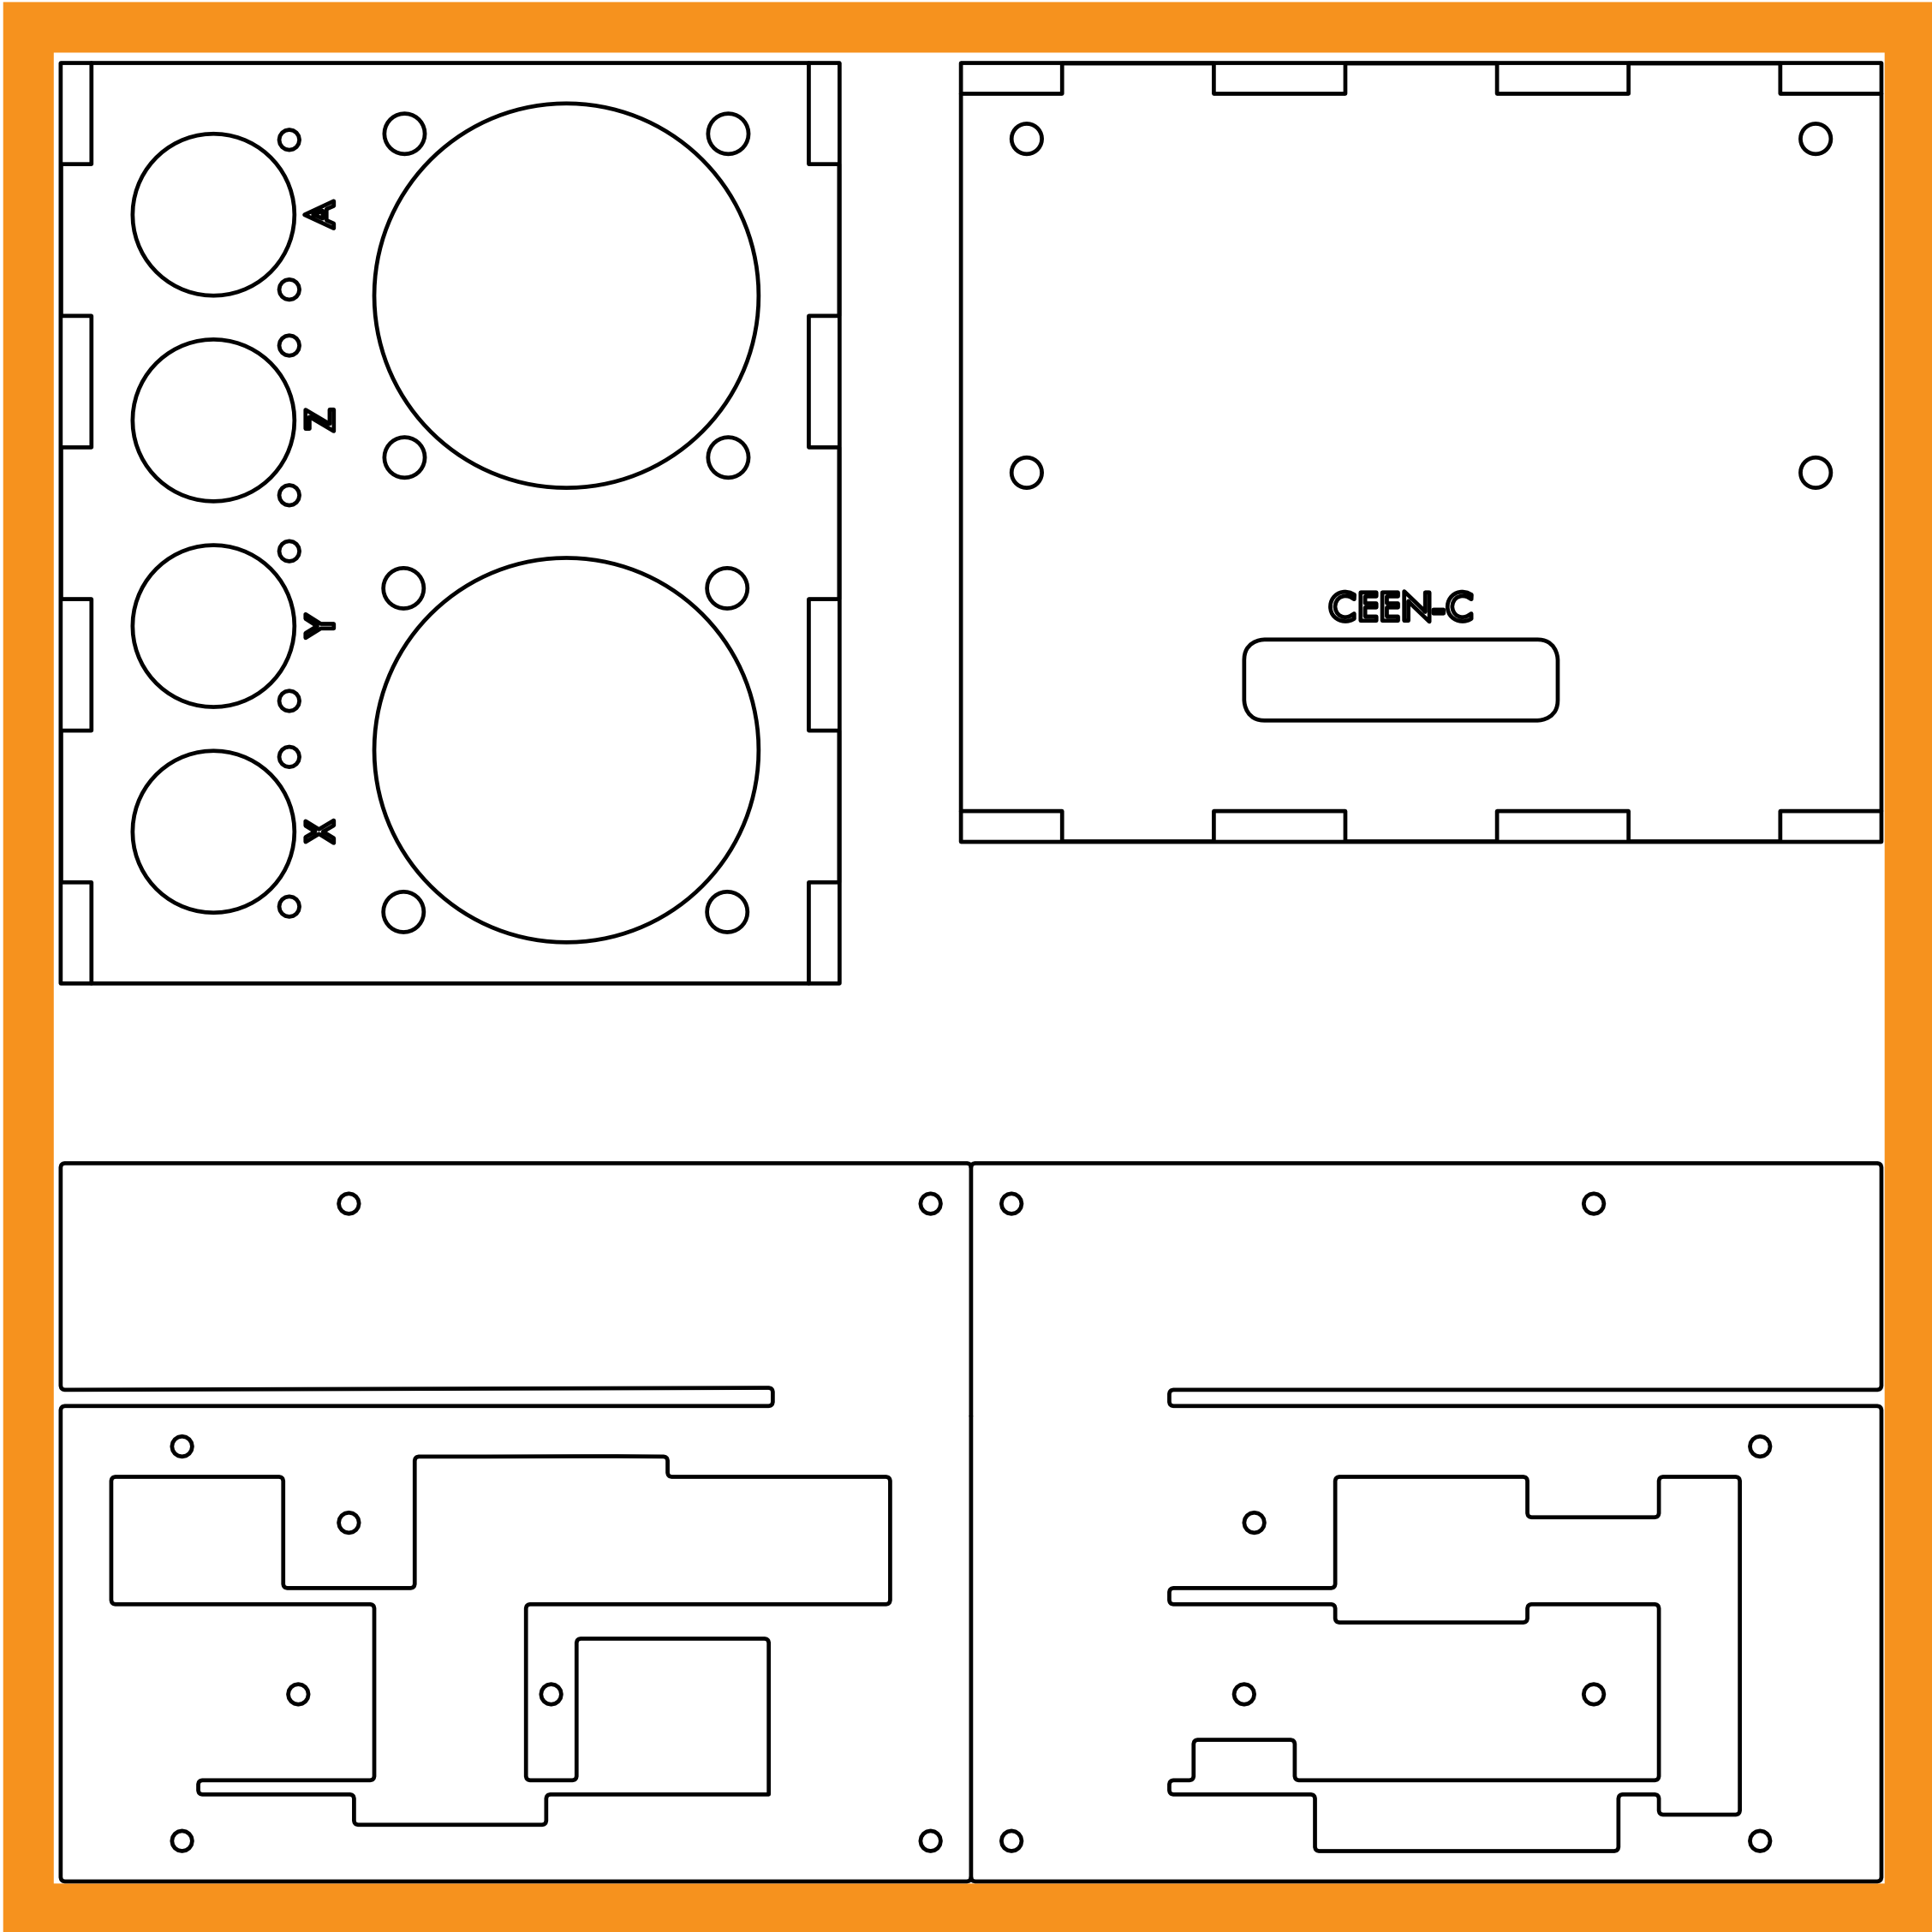
\includegraphics[width=1\textwidth]{packaging-design/front.png}
	\caption{Enclosure Front}
	\label{fig:front}
\end{figure}

\begin{figure}[h]
	\centering
	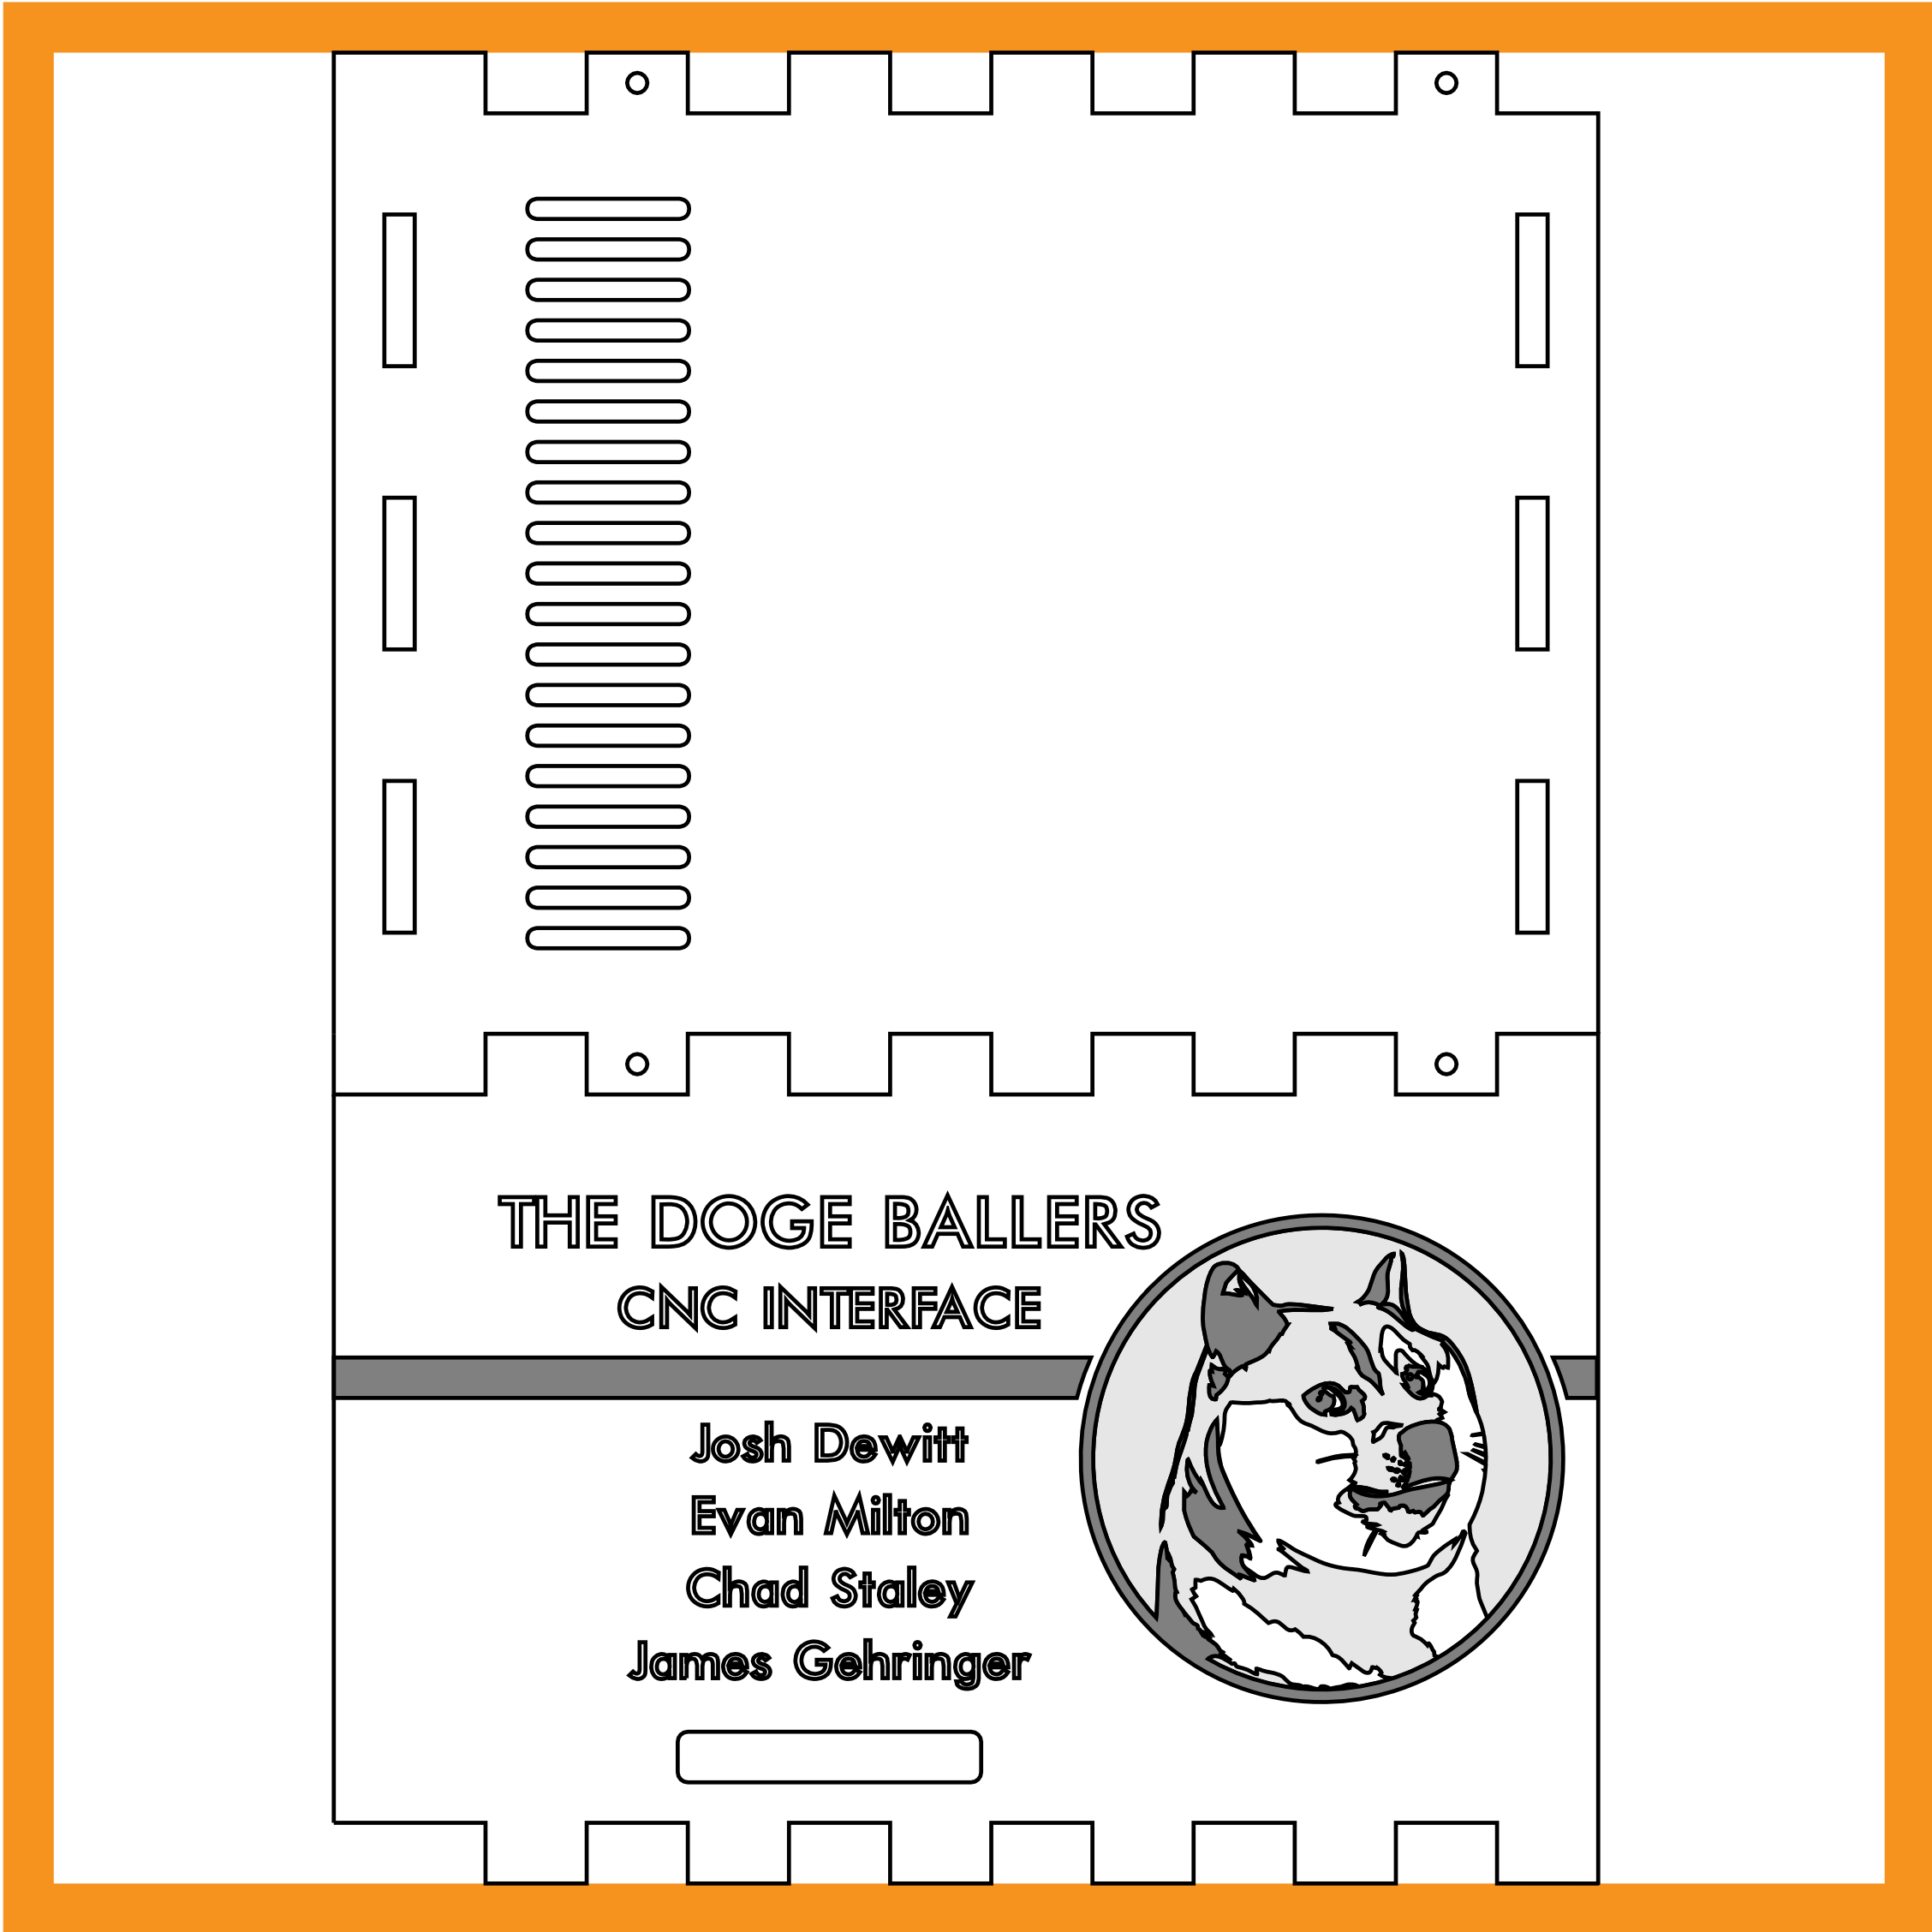
\includegraphics[width=1\textwidth]{packaging-design/side1.png}
	\caption{Enclosure Side Right}
	\label{fig:side1}
\end{figure}

\begin{figure}[h]
	\centering
	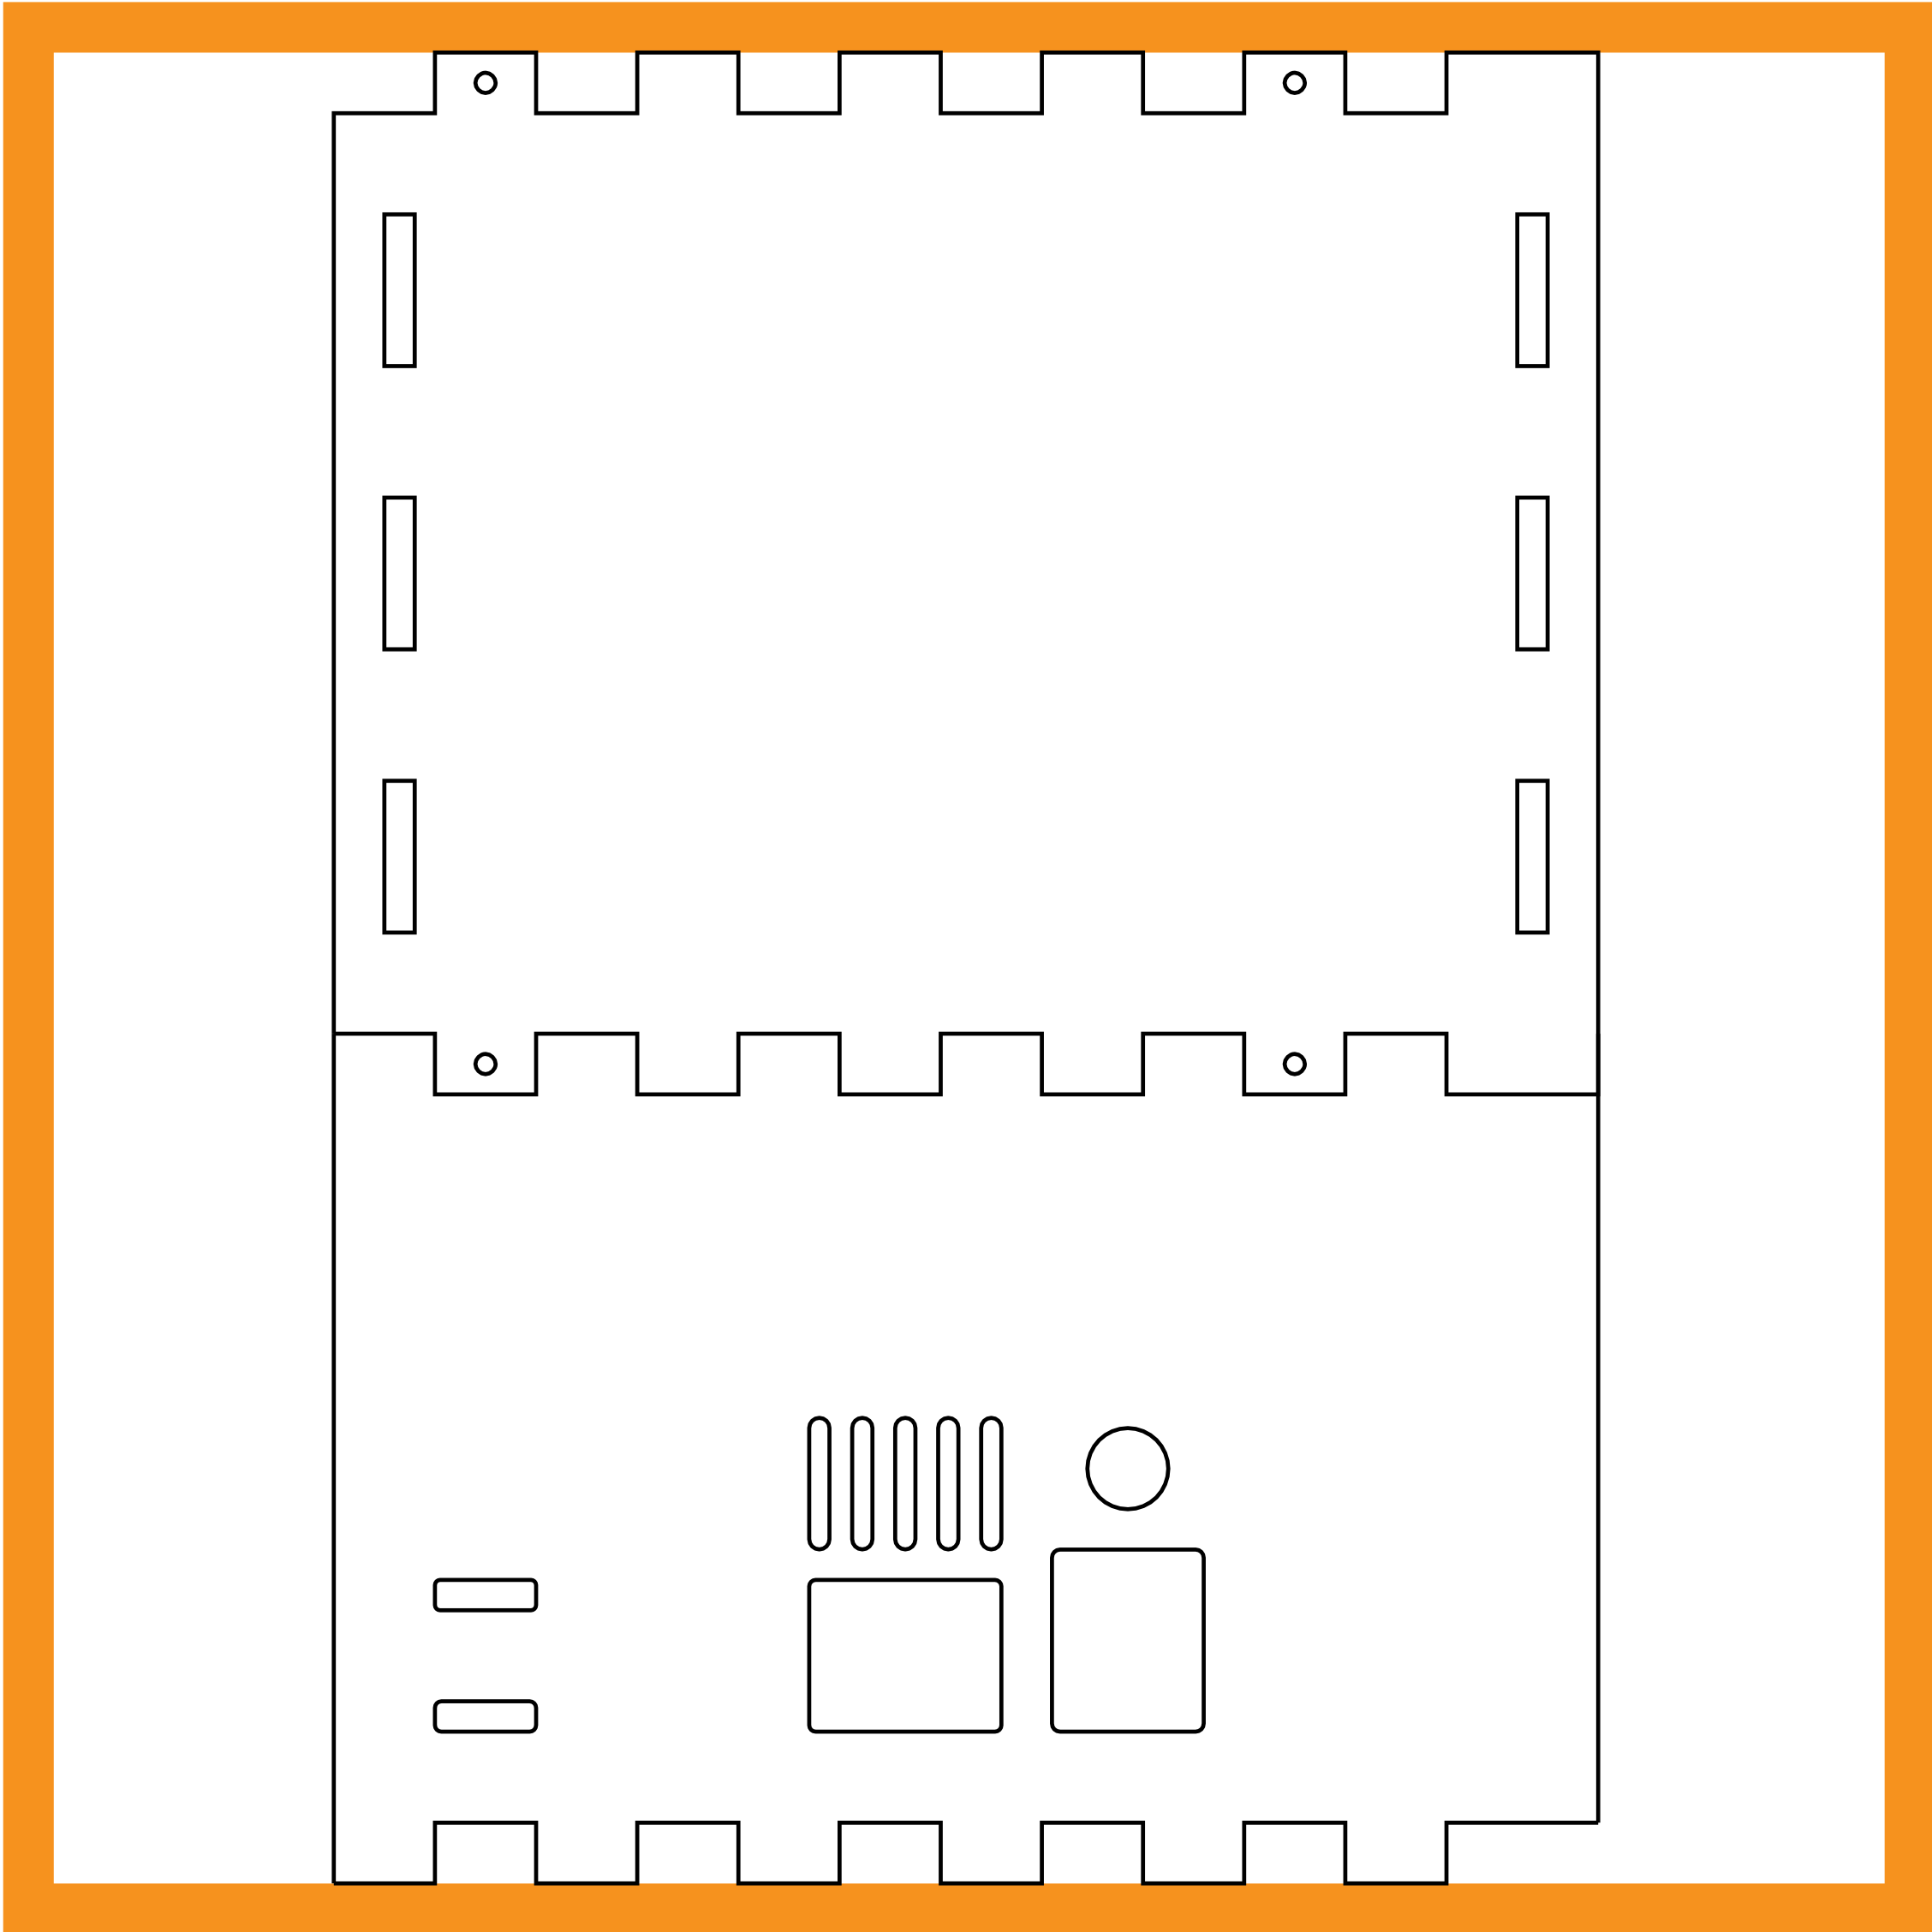
\includegraphics[width=1\textwidth]{packaging-design/side2.png}
	\caption{Enclosure Side Left}
	\label{fig:side2}
\end{figure}

\section{Hardware Design}

\subsection{Introduction}
The \gls{ceenc} consists of three major hardware components, the \gls{pi}, the control board, and the driver board.
The \gls{pi} will handle most of the processing and have a master relationship with the control board.
The control board will be an additional microcontroller that supports the \gls{pi} in timing and motor control functions.
The driver board will receive motor control commands from the control board and execute them using the \gls{ti} DRV8825 motor driver.
The driver board was developed and implemented separately from the control board to allow for early and individual testing.

\subsection{Raspberry Pi}
The \gls{pi} will receive G-code from the web interface over \gls{tcpip} through the Ethernet or USB ports.
The \gls{pi} will send commands to the motor control board microcontroller over a \gls{spi} bus.
The \gls{pi} will send data to a port expander on the control board over an \gls{i2c} connection.
The \gls{pi} will operate in the master mode for the \gls{spi} communication.
The control board will be dependent on the information it receives from the \gls{pi} for motor operation.
\gls{spi} was chosen because it is native on the \gls{pi} and most microcontrollers support it.
The \gls{pi} will be powered from the +5V rail on the control board.

\subsection{Control Board}
The control board will be implemented using the TI C2000 microcontroller.
A microcontroller supports the \gls{pi} so that the stepper motor timers can be run independently from the overhead of an operating system.
The microcontroller will receive commands from the \gls{pi} over a \gls{spi} connection.
The control board will contain an \gls{i2c} port expander that will provide 16 general purpose outputs and is controlled from the \gls{pi}.
The control board will send commands to the driver board over a parallel port connection.
A parallel port was chosen so that the driver board would also be able to interface with the parallel port on some PCs or other \gls{cnc} drivers.
The parallel port also allows for the I/O of the microcontroller to be mapped to the I/O of the motor drivers in a 1-to-1 relationship.
The microcontroller will output step, direction, and enable data for motor control.
It will receive fault and home inputs from the motor driver board.
The step lines must be capable of outputting a 10kHz signal.
A step frequency of 10kHz will be sufficient for \gls{cnc} applications.
The microcontroller uses 4 timers to track of the step count of each motor. 
The control board will have one DC power input.
This power input can range from 14V-36V.
There will be two regulated power supplies on the control board, 5V and 3.3V.
The 5V supply will power the \gls{pi}.
The 3.3V supply will power the microcontroller, the \gls{i2c} port expander, and the opto-isolators on the motor driver board.
The 14V-36V supply will power the motor drivers.

\subsection{Driver Board}
The motor drivers will be implemented using four \gls{ti} DRV8825.
The DRV8825 is a dual stepper/DC motor driver.
Each DRV8825 will receive step and direction commands from the motor control board over a parallel port connection.
The motor driver ICs will step the motors according to the commands from the microcontroller.
The motor driver board contains any necessary pull up/pull down resistors for the motor control signals.



\subsection{Summary}
\newpage
\section{Printed Circuit Board Design}
Standard \gls{pcb} design practices were implemented while designing the two custom \gls{pcb}s for this project.
The \gls{pcb} layout for the motor driver board is show in Figures ~\ref{fig:driver-top-cream} through ~\ref{fig:driver-bottom-copper}.

\subsection{Dimensions}
The \gls{ceenc} is based on the footprint of the \gls{pi}, and as such has stringent design requirements in terms of component layout and dimension.
\gls{gpio} headers must be carried across boards, as well as power connections and mounting points. Board length and width must also match that of the \gls{pi}. 

\subsection{Placement}
These requirements dictate the layout of major components, but leave many of the minor pieces unaccounted for.
After allocating areas for the microcontroller and power supply, major connectors are placed for optimal access to the remaining \gls{gpio}.
Indicator \gls{led}s, and test points are also placed for ease of use during the testing phase, and components are tweaked to provide an aesthetically pleasing, symmetrical layout.
The microcontroller is centrally located, to minimize trace lengths to the outlying components, reducing cross-talk and propagation delays.

\subsection{Power Considerations}
Power supply circuitry is isolated to a single section of the board, so as to limit the potential for interference.
Smoothing capacitors are placed as close as possible to the components for which they will be acting, and indicator \gls{led}s are used to mark active lines.
Larger trace widths are used for power lines as a rule of thumb, but of special consideration are the 10 Amp (instantaneous) lines to feed the driver board.
Positive and zero rails are also routed alongside one another, so as to counteract RF interferences that would otherwise result from the voltage differences.

\section{Software Design}

\subsection{Introduction}
The \gls{cnc} Interface is a project to drive a \gls{cnc} using a simple user interface and no need for installing drivers.
Additionally, the \gls{cnc} Interface will not be plugged into the computer, but will be controlled through the network instead.
The focus of software design for this project was to allow development from day one, not requiring any of the project's hardware to begin.
To achieve this goal, a test-driven development approach was adopted, meaning unit tests that verify project success are created before any application code is written.
This approach has allowed the software development to stay on track and not be pushed off until the end of the project.

\subsection{C2000 Software Design Considerations}
In this project, the \gls{ti} C2000 Piccolo microcontroller was chosen over the cheaper MSP430 because of more device support and available libraries.
The libraries provide an abstraction to the hardware registers allowing faster coding for the device. 

\subsubsection{Memory Model}
\begin{wraptable}{r}{8cm}
	\vspace{-18pt}
	\caption{C2000 Memory Map}
	\label{tab:memory-map}
	\centering
	{\footnotesize
	\begin{tabular}{rl|c|c|}
		\hline\hline
		&& Data Space & Program Space \\ \cline{3-4}
		0x00&0000 & \multicolumn{2}{c|}{M0 Vector RAM} \\ \cline{3-4}
		0x00&0040 & \multicolumn{2}{c|}{Boot Stack, RAM Functions} \\ \cline{3-4}
		0x00&0400 & \multicolumn{2}{c|}{Program Stack} \\ \cline{3-4}
		0x00&0600 & \multicolumn{2}{c|}{Global Variables} \\ \cline{3-4}
		0x00&0800 & Peripheral Frame 0 & Reserved \\ \cline{3-4}
		0x00&0D00 & Interrupt Table & Reserved \\ \cline{3-4}
		0x00&0E00 & Peripheral Frame 0 & Reserved \\ \cline{3-4}
		0x00&2000 & \multicolumn{2}{c|}{Reserved} \\ \cline{3-4}
		0x00&6000 & Peripheral Frame 1 & Reserved \\ \cline{3-4}
		0x00&7000 & Peripheral Frame 2 & Reserved \\ \cline{3-4}
		0x00&8000 & \multicolumn{2}{c|}{L0 SARAM} \\ \cline{3-4}
		0x00&9000 & \multicolumn{2}{c|}{Reserved} \\ \cline{3-4}
		0x3D&7800 & \multicolumn{2}{c|}{User OTP} \\ \cline{3-4}
		0x3D&7C00 & \multicolumn{2}{c|}{Reserved} \\ \cline{3-4}
		0x3F&0000 & \multicolumn{2}{c|}{Flash Program Code, Static Data} \\ \cline{3-4}
		0x3F&7FF6 & \multicolumn{2}{c|}{Flash Program Boot Location} \\ \cline{3-4}
		0x3F&7FF8 & \multicolumn{2}{c|}{128-bit Password} \\ \cline{3-4}
		0x3F&8000 & \multicolumn{2}{c|}{L0 SARAM} \\ \cline{3-4}
		0x3F&9000 & \multicolumn{2}{c|}{Reserved} \\ \cline{3-4}
		0x3F&E000 & \multicolumn{2}{c|}{Boot ROM} \\ \cline{3-4}
		\hline
	\end{tabular}
	}
\end{wraptable}
This slightly more expensive microcontroller has 12\gls{kb} of \gls{ram} and 64\gls{kb} of Flash allowing ample space for the project's code, along with 2\gls{kb} of \gls{otp} and 16\gls{kb} of factory-programmed \gls{rom} containing power-on boot-loading software and standard math-related tables, like sine and cosine waveforms.
Table~\ref{tab:memory-map} shows the C2000's memory map according to the datasheet\cite{piccolo} and the linker command file for the release configuration.
Note that each memory address is two bytes.
An alternate configuration exists that puts all code in \gls{ram}, but this configuration is only used for debugging because it is faster to load a new program into \gls{ram}.
Frequently executed code copied from flash into \gls{ram} at startup to allow power savings and ensure that it is fetched with 0 wait states on interrupt.

\subsubsection{C2000 Peripheral Usage}
The project makes use of the \gls{spi} for communication with the \gls{pi} during normal operation.
\gls{spi} was chosen because of the high-bandwidth achievable, already verified to work with a 1MHz clock using non-ideal wire jumpers.
The \gls{pi} communicates with the C2000 through \gls{uart} at startup for bootloader functions.
\gls{uart} was chosen because the boot \gls{rom} code defaults to interfacing with the \gls{uart} for serial bootloading.
\gls{gpio} pins are used to drive the direction lines for the motors, generate the stepper motor pulse trains, and read the status of the home and emergency stop signals.

\subsubsection{C2000 Code Architecture}
The C2000 code base uses a combination of polling the \gls{spi} communication device and timer-based interrupt-driven code for generating pulse trains to the motors.
A second interrupt is generated whenever the emergency stop line transitions from high-to-low or low-to-high, in which case all motor movement is stopped as quickly as possible.
The pulse train generation is real-time and must execute code as soon as the auto-reloaded timer expires, so polling for \gls{spi} data can be preempted by the timer interrupt.
An alternate design would be to use interrupt priority and allow the timer to interrupt the \gls{spi} interrupt, however a polling scheme is less risky and is easier to code.
Because communication can be interrupted, the \gls{pi} will require the C2000 to echo back sent data to ensure that the entire communication block was received.
Figure~\ref{fig:c2000-main} depicts the polling loop for the C2000 and figure~\ref{fig:c2000-pulse} depicts the interrupt routine for the pulse train generation.

\subsubsection{Raspberry Pi Code Architecture}
The code written for the \gls{pi} is written to read and write to named Linux pipes, or \gls{fifo} files managed by the \gls{os}.
These services are written to constantly run, so running a g-code file requires writing to a pipe, not starting up a program.
The use of pipes allows to better modularize the code base and avoid duplication by factoring out common code into projects.

\subsubsection{Testing and Debugging}
All code for the project is written after unit tests have been created that can be run on any machine using the program make to verify all application logic before implementing on the \gls{pi} or C2000.
The exception is writing to hardware configuration registers which must be changed, programmed, and manually tested for correctness.
Once these low-level configurations are created and verified, they are kept in a stable state in git and will not undergo unnecessary changes.
Code is considered complete when it passes all unit tests, that is, no code is written unless a failing tests proves that it is required.
It follows that new functionality requires that tests are written first, and code is written to make the tests pass.

\subsection{Software Design Narrative}
The code written for this project is intended to be as modular as possible, avoiding duplication of functionality and increasing testability.
The project relies on free software including the Arch distribution of Linux\cite{archlinux} for the \gls{os} on the \gls{pi}, Apache for web hosting from the \gls{pi}, PHP for creating the back-end services that the website makes calls to, JQuery for creating dynamic web pages, and CuTest, a lightweight unit testing framework for C projects.
As shown in figure~\ref{fig:firmware-hierarchy}, the project contains four software modules: the website control, g-code interpreter, \gls{cnc} driver, and the motor scheduler.
The bootloader on the C2000 is programmed into \gls{rom} and is thus not developed or maintained for this project.
Though not used during normal operation, a set of bash scripts grouped together to create a simple way to set up the \gls{pi} was created to be able to quickly set up the \gls{pi} and get ready for development.

\subsubsection{Website Control}
The website control project is written in HTML, CSS, JavaScript, and PHP and is the main interface between the user and the \gls{cnc}.
The website gives the user the ability to upload, delete, and run g-code files and configure the \gls{cnc}'s characteristics, like gearing ration, maximum speed, and maximum acceleration.
The website has been set up, outlined, and approximately 85\% written, with all written code being completely tested.

\subsubsection{g-code Interpreter}
The g-code interpreter project is written in C and is responsible for reading g-code line-by-line and interpreting it into instructions for the C2000 to generate the motor pulse trains.
The g-code interpreter listens to a pipe for g-code commands, which may come from a g-code file or directly from the website when the user is homing the machine, then writes to another pipe that is received by the \gls{cnc} driver.
At startup, the g-code interpreter is responsible for driving the state of the C2000, instructing it to home the \gls{cnc}.
The g-code interpreter relies heavily on mathematic formulas created by the software engineer, so many unit tests have been written to ensure proper functionality.
The g-code interpreter has been outlined, flow-charted, and approximately 90\% written, with all written code being completely tested.

\subsubsection{\gls{cnc} Driver}
The \gls{cnc} driver project is written in C and is responsible for managing communication channels between the \gls{pi} and C2000 through the \gls{spi} and \gls{uart}.
The g-code interpreter does not write to the \gls{spi} or \gls{uart} directly because these actions require root privileges, so this project was created to allow a single, small program to run as root, while the larger, more frequently changing programs are run by regular users.
The \gls{cnc} driver listens to a pipe for commands to send to the C2000 and forwards them through \gls{spi}, verifying that it is received based on the echo back from the C2000.
The \gls{cnc} driver also looks for a special command that indicates that the next bytes will be \gls{ti} hex data and the program should reset the C2000 and bootload the device with new code.
The \gls{cnc} driver has been outlined, flow-charted, and 100\% written and tested.

\subsubsection{Motor Scheduler}
The motor scheduler project is written in C and is responsible for listening for commands from the \gls{pi} and generating the pulse trains to the motors.
The project is based off an algorithm that requires no floating point operations on the C2000 for generating pulses, saving resources and allowing better real-time performance.
The commands are accepted through \gls{spi} and are acknowledged by echoing back the received data, with the command format specified in a C header file shared between the g-code interpreter and this project.
The motor scheduler has been outlined, flow-charted, and approximately 65\% written, with all written code being completely tested.

\subsection{Summary}
The \gls{cnc} Interface's software is currently on-time because of the development approaches involving test-driven development and well thought-out modular software architecture that makes changes simple and low-risk.
The software hierarchy is a modular design that takes advantage of the available features of the Linux \gls{os} for faster development.
To aid in rapid development and implementation all firmware upgrades to any component of the \gls{cnc} Interface can be made remotely.
A user can \gls{ssh} into the \gls{pi} and make changes to the website control, g-code interpreter, or \gls{cnc} driver projects directly and bootload new C2000 code over the \gls{uart}.
The software architecture created for this project is robust and encourages changes in improvements, while mitigating change risks through unit testing.


\section{Design Performance}
The product performs as expected.
All of the objectives were met.
When a mill is combined with a \gls{ceenc}, the mill correctly mills a design in a timely fashion. 
The general purpose outputs work correctly.
The system can drive four stepper motors, one DC motor, and receives input from an emergency stop switch and 4 stepper home inputs.
The g code used to execute commands can be sent over \gls{tcpip}.
The steppers are driven at a frequency range of at least 10kHz within 5\% accuracy.
The whole system can handle a variety of power supplies and draws no more than 10 amps.
The thermal shutdown also is triggered when the system reaches $60^{\circ}C$.